%\documentclass{sig-alternate-05-2015}
\documentclass{llncs}
\usepackage{makeidx}
\usepackage{tabularx,colortbl}
\usepackage[dvipsnames]{xcolor}
\usepackage{flushend}
\usepackage{cite}
\usepackage{amsmath}
%\usepackage{amsthm}
\usepackage{amssymb}
\usepackage{epsfig}
\usepackage{stmaryrd}
\usepackage{url}
\usepackage{multirow}
\usepackage{latexsym}
\usepackage{graphics}
\usepackage{graphicx}
\usepackage{enumitem}
\usepackage{comment}
\usepackage{longtable}
\usepackage{supertabular}
\usepackage{times}
\usepackage{listings}
\usepackage{subfigure}
\usepackage{color}
\usepackage{balance}
\usepackage{xspace}
\usepackage[ruled, vlined, linesnumbered]{algorithm2e}



%\theoremstyle{Definition}
%\newtheorem{definition}{Definition}
%%%
%\theoremstyle{Theorem}
%\newtheorem{theorem}{Theorem}


%\newcommand{\definition}{\noindent \textbf{Definition} \citation{}}
%\newcommand{\theorem}{\noindent \textbf{Theorem} \citation{}}
%\newcommand{\lemma}{\noindent \textbf{Lemma} \citation{}}

%\newdef{lemma}{Lemma}
%\newdef{definition}{Definition}
%\newdef{theorem}{Theorem}
%\newdef{corollary}{Corollary}
%\newdef{note}{Note}
%\newdef{axiom}{Axiom}
\newcommand{\mkeyword}[1]{\mbox{\texttt{#1}}}
\DeclareMathOperator{\kuop}{uop}
\DeclareMathOperator{\kbop}{bop}
\DeclareMathOperator{\kite}{ite}
\DeclareMathOperator{\kpre}{pre}
\DeclareMathOperator{\dom}{dom}
\DeclareMathOperator{\ktrue}{true}
\DeclareMathOperator{\kfalse}{false}
\DeclareMathOperator{\kselect}{select}
\DeclareMathOperator{\ran}{range}
\newcommand{\lbb}{[\![}
\newcommand{\rbb}{]\!]}
\newcommand{\expr}{\phi}
\newcommand{\exprS}{\Phi}
\newcommand{\mike}[1]{\textcolor{red}{#1}}
\newcommand{\mats}[1]{\textcolor{blue}{#1}}
\newcommand{\darren}[1]{\textcolor{green}{#1}}
\newcommand{\danielle}[1]{\textcolor{purple}{#1}}


\sloppypar



\begin{document}

\definecolor{gold}{rgb}{0.90,.66,0}
\definecolor{dgreen}{rgb}{0,0.6,0}
\newcommand{\stateequiv}{\equiv_{s}}
\newcommand{\traceequiv}{\equiv_{\sigma}}
\newcommand{\ta}{\text{TA}}
\newcommand{\cta}{\text{TA$_{C}$}}
\newcommand{\tta}{\text{TA$_{T}$}}
\newcommand{\ucalg}{\texttt{\small{IVC\_UC}}}
\newcommand{\ucbfalg}{\texttt{\small{IVC\_UCBF}}}


\title{Architectural Modeling and Analysis for Safety Engineering}
%
\author{Danielle Stewart\inst{1}
\and Michael W. Whalen\inst{1}
\and Mats Heimdahl\inst{1}
\and Darren Cofer\inst{2} }

\institute{University of Minnesota\\Department of Computer
Science and Engineering\\
200 Union Street\\
Minneapolis, MN, 55455, USA\\
\email{dkstewar, whalen, heimdahl@cs.umn.edu}
\and
Rockwell Collins\\
Advanced Technology Center\\400 Collins Rd. NE\\
Cedar Rapids, IA, 52498, USA\\ \email{ darren.cofer@rockwellcollins.com}
}
\maketitle

\begin{abstract}
Model-based systems engineering (MBSE) methods and tools permit system-level requirements to be specified and analyzed early in the development process of airborne and ground-based systems. These tools can also be used to perform safety analysis based on the system architecture and initial functional decomposition.

Previously, Rockwell Collins and the University of Minnesota developed and demonstrated an approach to model-based safety analysis. New MBSE tools that incorporate assume-guarantee compositional analysis techniques provide the basis for greatly improving earlier approaches to safety analysis and can be used to ensure model consistency, correctness of assumptions, and better scalability.

Using AADL-based system architecture modeling and analysis tools as an exemplar, we extend existing analysis methods to support system safety objectives of ARP4754A and ARP4761. This includes extensions to existing modeling languages to better describe failure conditions, interactions, and mitigations, and improvements to compositional reasoning approaches focused on the specific needs of system safety analysis. We develop example systems based on the Wheel Braking System in SAE AIR6110 to evaluate the effectiveness and practicality of our approach.
\end{abstract}

\keywords{Model-based systems engineering, fault analysis, safety engineering}

\section{Introduction}

System safety analysis techniques are well established and are a required activity in the development of commercial aircraft and safety-critical ground systems. However, these techniques are based on informal system descriptions that are separate from the actual system design artifacts, and are highly dependent on the skill and intuition of a safety analyst. The lack of precise models of the system architecture and its failure modes often forces safety analysts to devote significant effort to gathering architectural details about the system behavior from multiple sources and embedding this information in safety artifacts, such as fault trees.

While model-based development (MBD) methods are widely used in the aerospace industry, they are generally disconnected from the safety analysis process itself. Formal model-based systems engineering (MBSE) methods and tools~\cite{QFCS15:backes,hilt2013,NFM2012:CoGaMiWhLaLu,DBLP:journals/scp/CimattiT15,Pajic2012,DBLP:conf/adaEurope/SokolskyLC09} now permit system-level requirements to be specified and analyzed early in the development process. These tools can also be used to perform safety analysis based on the system architecture and initial functional decomposition. Design models from which aircraft systems are developed can be integrated into the safety analysis process to help guarantee accurate and consistent results. This integration is especially important as the amount of safety-critical hardware and software in domains such as aerospace, automotive, and medical devices has dramatically increased due to desire for greater autonomy, capability, and connectedness.

Architecture description languages, such as SysML~\cite{SysML} and the Architecture Analysis and Design Language (AADL)~\cite{AADL} are appropriate for capturing system safety information.  There are several tools that currently support reasoning about faults in architecture description languages, such as the AADL error annex~\cite{Larson:2013:IAE:2527269.2527271} and HiP-HOPS for EAST-ADL~\cite{CHEN201391}.  However, these approaches primarily use {\em qualitative} reasoning, in which faults are enumerated and their propagations through system components must be explicitly described.  Given many possible faults, these propagation relationships become complex and it is also difficult to describe temporal properties of faults that evolve over time (e.g., leaky valve or slow divergence of sensor values).

In earlier work, University of Minnesota and Rockwell Collins developed and demonstrated an approach to model-based safety analysis (MBSA) \cite {Joshi05:Dasc,Joshi05:SafeComp,NasaRep:MBSA-Aug05} using the Simulink notation \cite{MathWorks}.  In this approach, a behavioral model of (sometimes simplified) system dynamics was used to reason about the effect of faults.  We believe that this approach allows a natural and implicit notion of fault propagation through the changes in pressure, mode, etc. that describe the system's behavior.  Unlike qualitative approaches, this approach allows uniform reasoning about system functionality and failure behavior, and can describe complex temporal fault behaviors.  On the other hand, Simulink is not an architecture description language, and several system engineering aspects, such as hardware devices and non-functional aspects cannot be easily captured in models.

\iffalse
Over the last five years, several research groups have focused on formal reasoning at the system architecture level, resulting in MBSE tools that incorporate assume-guarantee compositional reasoning techniques~\cite{Trento and Rockwell and UMN}.  These tools allow behavioral reasoning about complex system models, but with substantially greater scalability than previous approaches.
\fi

This paper describes our initial work towards a behavioral approach to MBSA using AADL.  Using assume-guarantee compositional reasoning techniques, we hope to support system safety objectives of ARP4754A and ARP4761.  To make these capabilities accessible to practicing safety engineers, it is necessary to extend modeling notations to better describe failure conditions, interactions, and mitigations, and provide improvements to compositional reasoning approaches focused on the specific needs of system safety analysis.  These extensions involve creating models of fault effects and weaving them into the analysis process.  To a large extent, our work has been an adaptation of the work of Joshi et. al to the AADL modeling language.

To evaluate the effectiveness and practicality of our approach, we developed an architectural model of the Wheel Braking System model in SAE AIR6110.  Starting from a reference AADL model constructed by the SEI instrumented with qualitative safety analysis information~\cite{SEI:AADL}, we added behavioral contracts to the model.  In so doing, we determine that there are errors related to (manually constructed) propagations across components, and also an architecture that contains single points of failure.  We use our analyses to find and fix these errors.

The rest of the paper is organized as follows...





\section{Model-Based Safety Analysis}

\mike{Audience should already know about model-based safety analysis.  We want to discuss two ``strands'' of MBSA, one with explicit fault propagation of faults rather than system dynamics, and another based on faults propagating through their effects on dynamics}.

A model-based approach for safety analysis was first proposed by Joshi et. al in \cite{Joshi05:Dasc, Joshi05:SafeComp, Joshi07:Hase}.  In this approach, a safety analysis system model (SASM) is the central artifact in the safety analysis process, and traditional safety analysis artifacts, such as fault trees, are automatically generated by tools that analyze the SASM. Figure~\ref{fig:sasm} provides an overview of this process applied to the wheel braking system example.

The contents and structure of the SASM differ significantly across different conceptions of MBSA.  We can draw broad outlines between two different approaches: one in which {\em faults} are propagated between components explicitly and the analysis proceeds by determining the likelihood of faults to system boundaries, and another in which faults propagate by changing the system dynamics, which may cause the system behavior to visibly change.  We call the first style the {\em explicit fault propagation} and the second style {\em implicit fault propagation} or {\em behavioral} propagation.

We contrast these two styles below...

\mike{Regurgitate content from "Model-Based Safety Analysis with smartIflow"}
\danielle{I added the citation from this paper to the bib file: cite\{info17:HaLuHo\} in case we want to use it.} \cite{info17:HaLuHo}.

\mike{Some contrasting points: richness of dynamics.  Most tools use formalisms that can only represent discrete quantities; we can do real-valued or large-domain integer dynamics}


\mike{Also we are explicitly integrated with an architecture language}


\subsection{Explicit Fault Propagation Approaches}



\mike{What is being done in AltaRica, HiPHOPS, AADL Error Annex...more here about primacy of faults as the mechanism of propagation between components.  Steal from proposal.}
\danielle{I added a few things from the proposal regarding fault propagation between components. There is a note below where that begins. I am not sure which papers you are referring to here so I can't really dig into those...}

The explicit propagation approach focuses on faults rather than constructing a model of system dynamics.

We illustrate this approach with the AADL error model annex~\cite{SAEAS} that can be used to describe system behaviors in the presence of faults. This annex has facilities for defining error types which can be used to describe error events that indicate errors in the system. The behavior of system components in the presence of errors is determined by state machines that are attached to system components; these state machines can determine error propagations and error composition for systems created from various subcomponents.

Error types in this framework are a set of enumeration values such as NoData, BadData, LateDelivery, EarlyDelivery, TimingError, and NoService. These errors can be arranged in a hierarchy. For example, LateDelivery and EarlyDelivery are subtypes of TimingError. The errors do not have any information (other than their type) associated with them. AADL includes information on the bindings of logical components (processes, threads, systems) and their communication mechanisms onto physical resources (memories, processors, busses), and the error annex uses this information to describe how physical failures can manifest in logical components.

\begin{figure}
  \centering
 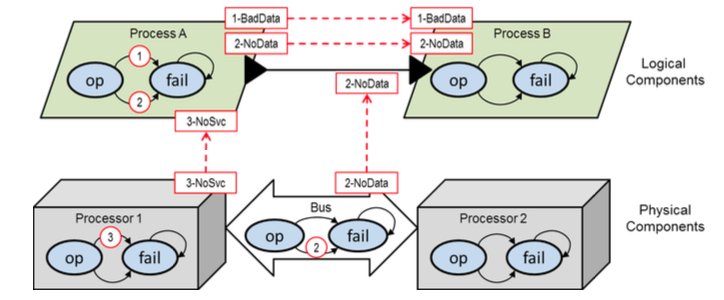
\includegraphics[width=0.75\textwidth]{images/error_annex.png}
  \vspace{-0.1in}
  \caption{Example of Error Model Information and Propagation}
  \label{fig:error_annex}
\end{figure}

An example is shown in Figure~\ref{fig:error_annex} \mike{Where is this figure?!?} \danielle{It was in the MBSA section. I have moved it here and if needed will reference from there}. Errors are described by the red rectangles labeled with error types: 1-BadData, 2-NoData, 3-NoSvc. Error events that can cause a component to fail are labeled with the corresponding error number. The error behavior of components is described by their state machines. Note that while all state machines in Figure 2 have two states, they can be much more complex. The red dashed arrows indicate propagations describing how failures in one component can cause other components to fail. For example, failures in the physical layer propagate to failures in the associated logical components.

Although the error model annex is very capable, it is not closely tied to the behavioral model of components or their requirements. For example, in the wheel braking system (WBS) example \cite{AIR6110}, it is possible that hydraulic system valves can fail open or fail closed. In fail closed, downstream components receive no flow and upstream pipes may become highly pressurized as a natural consequence of the failure. Physical models of these behavioral relationships often exist that can propagate failures in terms of the behavioral relationships between components. However, with the AADL error model annex, the propagations must be (re)specified and defined for each component. The user must therefore model the system twice, specifying propagations in the models of the physical phenomena, and again using enumerations and propagation rules in state machines in the error model annex. This re-specification can lead to inconsistencies between physical models and error annex models. In addition, the physical relationships between failures can be complex and may not be describable using enumeration values, leading to additional inconsistencies between the behavior of the physical phenomenon and the behavior of the error model.

\danielle{Added from proposal. I believe this describes what you mentioned above, Mike.}
This research attempts to bridge the descriptions of errors in the error model annex with behavioral descriptions of components. We start from the error model notions of error types and state machines that describe transitions from nominal to error states. However, we then tie these nominal and error states to behavioral models of the components in question that describe how the faults manifest themselves in terms of the signals or quantities produced by the components. Now the behavioral models can provide implicit propagation of the faulty behaviors and the natural consequences of failures on component behavior will be manifested in the propagation of other component faults through the behavioral model.

To accomplish this, we use AADL and the error model annex to describe faults and to use the AGREE contract specification language to describe behavioral models. This will require extensions to AGREE to define fault models that describe how different faults manifest themselves in changes to output signals. It will also require changes to the error annex. The conditions under which faults occur will become richer such that they describe not just propagation of enumerations from other components, but also valuations of input signals. For example, very high pressure in a pipe in the WBS model may lead to a \textit{pipe burst} failure. 


\subsection{Implicit Fault Propagation Approaches (Behavioral MBSA)}

\mike{Unfortunately, this is what is done, and done well in xSAP; they have a CAV paper on it; need to account for this}.
\danielle{I have been trying to find this paper... not sure what it is. I will move on for now and perhaps you have the paper title so that I can add a citation and some accounting for their research.}

The analysis starts from a {\em nominal} model of the system that describes the system behavior when no faults are present.  To perform safety analysis, we then also formalize the fault model. The fault model, in addition to common failure modes like \emph{non-deterministic}, \emph{inverted}, \emph{stuck\_at} etc, could encode information
regarding fault propagation, simultaneous dependent faults and fault hierarchies, etc.
After specifying the fault model and composing it with the original system model, the safety analysis involves verifying whether the safety requirements hold in presence of the faults defined in the fault model.


In this work, a behavior fault modeling language was constructed as an extension to the Lustre language \cite{Halbwachs91:IEEE}. Lustre is the kernel language of the popular model-based development tool SCADE \cite{SCADE}. In this approach, a safety engineer can model different kinds of fault behavior: e.g., stuck-at, ramp-up, ramp-down, and nondeterministic, and then {\em weave} these fault models into the nominal model. The language for describing faults is extensible, allowing engineers to define a catalog of faults appropriate for their domain. In addition, the weaving process allows error propagation between unconnected components within a system model \cite{Joshi07:Hase}. This allows consideration of physical aspects (e.g., proximity of components, shared resources such as power) that may not be present in a logical system model but can lead to dependent failures. In addition, it allows propagation of faults in the reverse direction of the model data flow. This can occur when physical components have coupling such as back-pressure in fluid systems or power surges in the opposite direction of communication through connected components. Finally, it is possible to create fault mediations to describe the output in the presence of multiple simultaneous faults.



%In previous work, component-level modeling tools such as Simulink \cite{MathWorks} and SCADE \cite{SCADE} were extended. In this work, we adapt this process to target system architecture models \cite{AADL, SysML} for safety analysis.

%\subsection{Safety Analysis Approach}
\begin{figure}
  \centering
 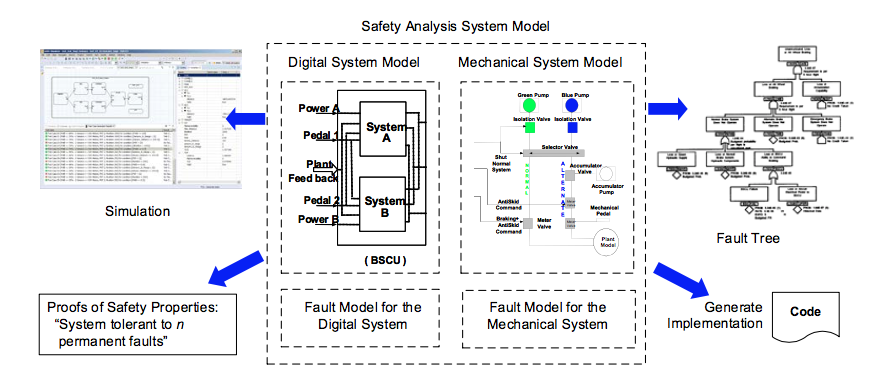
\includegraphics[width=1\textwidth]{images/SASM.png}
  \vspace{-0.1in}
  \caption{Safety Analysis System Model}
  \label{fig:sasm}
\end{figure}

A safety analysis system model can be used for a variety of simulations and analyses as shown in Figure~\ref{fig:sasm} \mike{include figure?} \danielle{Do you mean a figure like this one? If not, I can change it (I got it from the proposal) If so, perhaps Darren has a nonblurry copy of the figure? I can't get this one to be more clear...}. Modeling allows trivial exploration of \textit{what-if} scenarios involving combinations of faults through simulations. For more rigorous analyses, static analysis tools, such as model checkers and theorem provers, can be used to automatically prove (or disprove) whether the system meets specific safety requirements.
The primary approach used for analysis in previous work was model checking. After creating the system model, a model checker was used to verify that safety properties hold on the nominal system, an idealized model of the digital controller and the mechanical system containing no faults. Once the nominal model is shown to satisfy the safety property, the behavior of the fault-extended model can be examined. In the approach described by Joshi et al. in \cite{Joshi05:Dasc, Joshi05:SafeComp, Joshi07:Hase}, this analysis was performed by determining whether the property held for a given fault threshold: the maximum number of component faults to which the system is expected to be resilient.

This fault threshold is, in some sense, an approximation of the likelihood of component faults. It maps from the probabilistic \textit{real world} potential for component failure into a non-probabilistic verification problem. Recent work \cite{CAV2015:BoCiGrMa} uses a more sophisticated approach involving minimum cut sets to describe the set of potential component failures that must be considered. Both approaches provide separation between the probabilistic aspects of the real world and the computational demands of formal analysis. This approach currently scales far better than direct use of probabilistic model checking tools such as PRISM \cite{CAV2011:KwNoPa}, and will likely continue to do so in the future.

\iffalse
\subsection{Compositional Verification of System Architectures}

As part of the NASA Compositional Verification of Flight Critical Systems (CVFCS) project and the DARPA META and High Assurance Cyber Military Systems (HACMS) projects, we have constructed sophisticated compositional verification tools for reasoning about complex systems architectures. These tools \cite{NFM2012:CoGaMiWhLaLu} allow scaling of formal verification through splitting the analysis of a complex system architecture into a collection of verification tasks that correspond to the structure of the architecture. By decomposing the verification effort into proofs about each subsystem within the architecture, the analysis has been scaled to very large system designs \cite{QFCS15:backes}. In the case of the software for a complex medical drug infusion pump, a monolithic analysis of the design does not terminate in 24 hours, while the compositional approach completes in just over five minutes.
<<<<<<< HEAD
The approach naturally supports an architecture-based notion of requirements refinement based on assume-guarantee contracts. The properties of components necessary to prove a system-level property, including any assumptions about the component environment, in effect define the requirements for those components. The approach allows reuse of the verification that must already be performed on safety-critical software components and enables distributed development by establishing the formal contracts for components that are used to assemble a system architecture. If we are able to establish a system property using only the contracts of its components, we have the means for performing virtual integration of the components. We can use the contract of each component as a specification for suppliers and have a great deal of confidence that if all the suppliers meet their specifications, the integrated system will work properly.
We have implemented this assume-guarantee mechanism for compositional verification as an extension of the AADL language derived from the safety property subset of the property specification language (PSL) \cite{IEEE:PSL}. The Assume-Guarantee Reasoning Environment (AGREE) is our tool for compositional verification of these contracts. Under the CVFCS project, we are currently adding automated bi-directional translation between AGREE contracts and implementation-level properties in languages such as C and Simulink. Initially, we will support translation into MATLAB properties for analysis using the Simulink Design Verifier and C assertions for analysis using source code model checkers (such as CMBC) or test- based verification. Since contracts are abstractions of component implementations, they provide a much more efficient way of representing heterogeneous components in the system model than translating the component models themselves.
=======

The approach naturally supports an architecture-based notion of requirements refinement based on assume-guarantee contracts. The properties of components necessary to prove a system-level property, including any assumptions about the component environment, in effect define the requirements for those components. The approach allows reuse of the verification that must already be performed on safety-critical software components and enables distributed development by establishing the formal contracts for components that are used to assemble a system architecture. If we are able to establish a system property using only the contracts of its components, we have the means for performing virtual integration of the components. We can use the contract of each component as a specification for suppliers and have a great deal of confidence that if all the suppliers meet their specifications, the integrated system will work properly.

We have implemented this assume-guarantee mechanism for compositional verification as an extension of the AADL language derived from the safety property subset of the property specification language (PSL) \cite{IEEE:PSL}. The Assume-Guarantee Reasoning Environment (AGREE) is our tool for compositional verification of these contracts. Under the CVFCS project, we are currently adding automated bi-directional translation between AGREE contracts and implementation-level properties in languages such as C and Simulink. Initially, we will support translation into MATLAB properties for analysis using the Simulink Design Verifier and C assertions for analysis using source code model checkers (such as CMBC) or test- based verification. Since contracts are abstractions of component implementations, they provide a much more efficient way of representing heterogeneous components in the system model than translating the component models themselves.

>>>>>>> 705062d4005b55c503d3e85e228be8e236a1ac1e

\fi



\section{New MBSA Capabilities}

\mike{REWRITE!}

Previous research has been based on MBD tools (such as Simulink and SCADE) that were available at the time \cite{Joshi05:Dasc}. However, these tools are really targeted at the design and implementation of software components, rather than at the system architecture level where most safety concerns arise.

Within the past five years there have been great advances in the capabilities of tools for modeling and analysis of at the system level, based on languages such as SysML \cite{SysML} and AADL \cite{AADL}. We use these new MBSE capabilities and extend them to implement the safety analysis methods needed for the design and certification of commercial aircraft systems. The system modeling tools that we plan to use are based on AADL, but they can import and export models from SysML.

\begin{itemize}
\item We will improve the efficiency of MBSA methods by using MBSE tools that can perform compositional reasoning over complex system models. Using the assume- guarantee contract mechanism, these tools provide support for heterogeneous component models implemented in different languages (such as Simulink or C/C++).

\item Our new analysis methods move away from traditional static safety analysis methods focused on probabilistic models (e.g., Fault Tree Analysis), to the direct modeling of potential failure mechanisms and the analysis of dynamic fault-mitigation strategies.

\item Formal verification of system models provides increased assurance that these models are accurate and will produce correct results. The hierarchical structure of system architecture models supports analysis at varying levels of abstraction. Compositional analysis explicitly checks assumptions captured in component and subsystem contracts. Consistency and realizability checks [23] provide the ability to detect conflicting requirements between component and subsystem models.
\end{itemize}

%In this section we describe some of the new capabilities that we will develop, including improvements related to the AADL Error Model Annex, the use of model-based assurance cases, and evaluation of system-level certification objectives related to system safety that can be satisfied using the proposed methods.
\danielle{Removed the sections that were written in the safety.tex portion of the paper.}
%We bridge the descriptions of errors in the error model annex with behavioral descriptions of components. We start from the error model notions of error types and state machines that describe transitions from nominal to error states. However, we then tie these nominal and error states to behavioral models of the components in question that describe how the faults manifest themselves in terms of the signals or quantities produced by the components. Now the behavioral models can provide implicit propagation of the faulty behaviors and the natural consequences of failures on component behavior will be manifested in the propagation of other component faults through the behavioral model.

%To accomplish this, we use AADL and the error model annex to describe faults, and to use the AGREE contract specification language to describe behavioral models. This requires extensions to AGREE to define fault models that describe how different faults manifest themselves in changes to output signals. It also requires changes to the error annex. The conditions under which faults occur will become richer such that they describe not just propagation of enumerations from other components, but also valuations of input signals.





%\subsection{Fault and Behavioral Modeling}



\section{ARP4761: Wheel Brake System}

%\mike{Move the generic description to a section right after the ``safety'' section along with the ARP figure.  Leave the modeling that we did in AADL here.  That way we can reference it in the MBSA sections.}
%\danielle{The whole nominal model description is here. The modeling we did is in the faults section.}

As a preliminary case study, we utilized the Wheel Brake System described in ARP 4761 - Appendix L \cite{AIR6110}. The Wheel Brake System is installed on the two main landing gears and is used during taxi, landing, and rejected take off. Braking is either commanded manually using brake pedals or automatically with no need for the pedals (autobrake). When the wheels have traction, the autobrake function will provide a constant smooth deceleration.

%%%%%%%%%%%% Try to get a better figure here... this one is all blurry...
\begin{figure}
\begin{center}
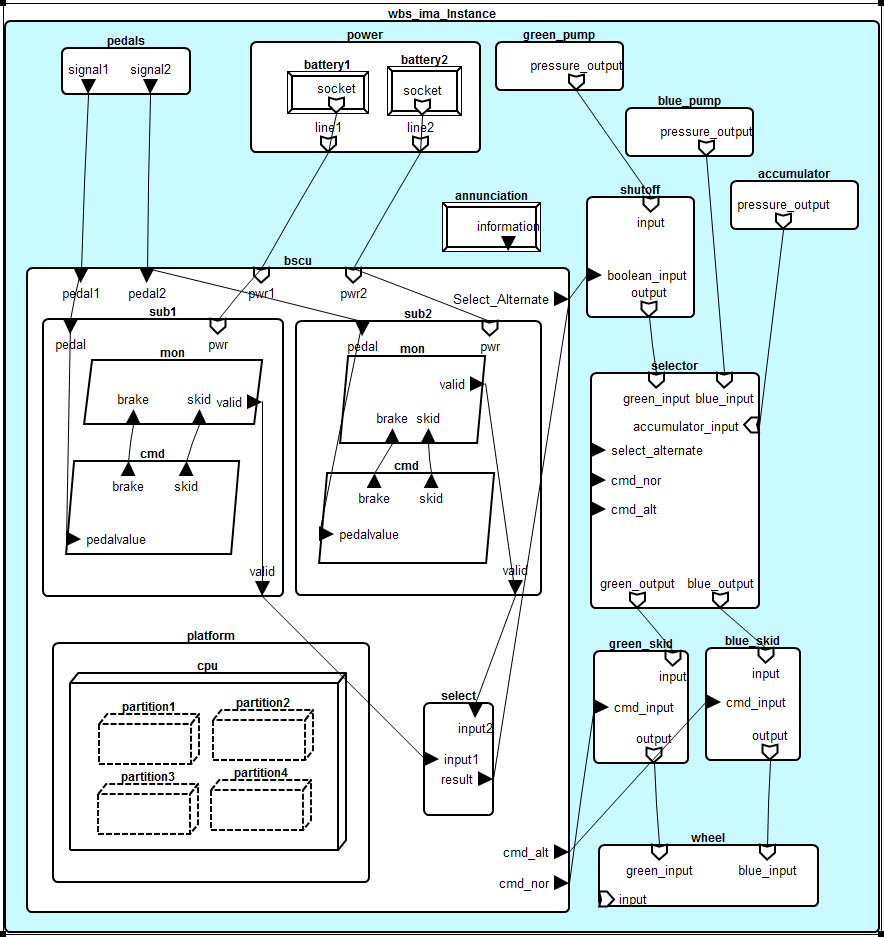
\includegraphics[scale=.5]{images/Wbs-ima.png}
\caption{AADL Simple Model of the Wheel Brake System }\label{fig:wbs_ima}
\mike{NOTE: selector::select\_alternate is not connected (we fixed this in our model)}
\mike{maybe we could add the modified portion of the model into the figure}
\danielle{The connection is added.}
\end{center}
\end{figure}

Each wheel has a brake assembly that is operated by two sets of hydraulic pistons which operate independently. One set is operated by the Green hydraulic line which is used in Normal braking mode. The second system (Alternate) is operated by the Blue hydraulic line which is used when the Normal system fails. The Alternate system is also supplied by an Accumulator which is a device with built up pressure that can be released if both of the two primary pumps (Blue and Green) fail. The accumulator supplies the Alternate system in case of Emergency braking mode.

Switching between the hydraulic pistons and sources can be done automatically or manually. If the Normal pressure (Green) is below a certain threshold, there is an automatic switchover to the Blue supply. If the Blue pump fails, then the Accumulator is used for hydraulic pressure.

In both Normal and Alternate modes, an anti-skid capability is available. In the Normal mode, the brake pedal position is electronically fed to a braking computer called the Braking System Control Unit (BSCU). The BSCU monitors signals that denote critical aircraft and system states to provide correct braking function, detect anomalies, broadcast warnings, and sent maintenance information to other systems.

\subsection{Nominal System Modeling}
A formal specification of the nominal system model consists of mechanical and digital components and their interconnections. Figure~\ref{fig:wbs_ima} illustrates how the wheel braking system is modeled using Architecture Analysis and Design Language (AADL). The following section describes this nominal model from which the fault model was generated.

\paragraph{Wheel Braking System (WBS)}
The highest level component is the WBS. It consists of a digital control unit, the BSCU, and Normal and Alternate hydraulic pressure lines (supplied by Green Pump and Blue Pump/Accumulator respectively), a Selector which selects between Normal and Alternate modes of hydraulic pressure, and the Wheel system. The WBS takes inputs from the environment including PedalPos1, AutoBrake, DecRate, AC\_Speed, and Skid. All of these inputs are forwarded to the BSCU to compute the brake commands.

\paragraph{Braking System Control Unit (BSCU)}
The BSCU is the digital component in the system that receives inputs from the WBS. It also receives feedback from the Normal and Alternate lines and two power inputs from two separate power sources. The BSCU is composed of two Command and Monitor subsystems each powered independently from separate power sources. The pedal position maps into these units and when skidding occurs, the Command and Monitor units will decrease the pressure to the brakes.

The Command unit regulates the pressure to the brakes in the Normal hydraulic line through the command cmd\_nor. Computing this command requires both the brake requested power and the skid information. The Command unit also regulates the pressure in the Alternate hydraulic line in order to prevent skidding which it does through the cmd\_alt command. The Monitor unit monitors the validity of the Command unit output.

The BSCU switches to the Alternate hydraulic system under the following conditions:
\begin{itemize}
\item Output from both Command units are not valid
\item The Green pump (Normal) is below threshold
\end{itemize}

\noindent Once the system has switched into Alternate mode, it will not switch into Normal mode again.

\paragraph{Hydraulic Pumps}.
There are three hydraulic pumps in the system, Green pump (Normal mode), Blue pump (Alternate mode), and Accumulator pump (Emergency mode). Each pump provides pressure to the system and is modeled in AADL as a floating point value.

\paragraph{Shutoff Valve}
%%%%%%%%%%%%%%%%%% Look at this more closely in wbs.aadl %%%%%%%%%%

The Shutoff valve is a meter valve situated between the Green pump and the Selector. It receives an input from the BSCU regarding valve position and regulates the pressure coming through the Green pipe accordingly.

\paragraph{Selector Valve}
The selector receives inputs from the pumps regarding pressure output and the BSCU regarding which mode the system is in. It will output the appropriate pressure from Green, Blue, or Accumulator pump. An added requirement of the Selector system is that it will only output pressure from one of these sources. Thus, the case of having pressure supplied to the wheels from more than one pump is avoided. The Selector takes the two pipe pressures (Green and Blue) as input, selects the system with adequate pressure and blocks the system with inadequate pressure. It is unclear how the Selector valve operates if both incoming pipes have pressure greater than the threshold. The AADL model assumes that the default in this case is Normal mode.

\paragraph{Skid Valves}
The Blue\_Skid and Green\_Skid valves receive input from the Selector as pressure coming through the respective pipes as well as input from the BSCU that commands Normal or Alternate mode. The Skid valves will use these inputs to choose between the Green or the Blue pressure to send off to the wheel.


\iffalse

\subsection{Nominal System Modeling}
\mike{KEEP HERE!}
A formal specification of the nominal system model consists of mechanical and digital components and their interconnections.

The highest level component is the Wheel Braking System (WBS). It consists of a digital control unit, the BSCU, and Normal and Alternate hydraulic pressure lines (supplied by Green Pump and Blue Pump/Accumulator respectively). The system takes inputs from the environment including PedalPos1, AutoBrake, DecRate, AC\_Speed, and Skid. All of these inputs are forwarded to the BSCU to compute the brake commands. The outputs of the WBS are Normal\_Pressure, Alternate\_Pressure, and System\_Mode (NORMAL, ALTERNATE, EMERGENCY).

\subsection{Braking System Control Unit (BSCU)}
The BSCU is the digital component in the system that receives inputs from the WBS. It also receives feedback from the Normal and Alternate lines and two power inputs from two separate power sources.

\fi



\section{Fault Modeling}

In order to start from the error model notions of error types and look more closely at the state machines that describe transitions from the nominal state to the error state, we focus on the types of errors that can be present in the components of the system. 

To begin with, we proved a top level property of the WBS using AGREE. This property states: \\

\begin{tt}
If pedals are pressed and no skid occurs, then the brakes will receive pressure. \\
\end{tt}

Using the AADL nominal model, this property proves. From this point, we focus our attention on component failures and how this will affect the top level property of the system. 

We would like to specify different component failure modes. These failure modes can be triggered by some internal error or propagated fault. In order to trigger these faults, additional input was added to the AADL model for each fault that can occur within a nominal model component. Our simple fault model contains two types of faults:

\begin{itemize}
\item \textit{fail\_to} fault: This type of failure accounts for both nondeterministic failures and stuck-at failures. The components that are affected by this fault include meter valves and pumps. This fault can be modeled in such a way as to describe both digital and mechanical errors. Examples of digital errors include a \textit{stuck\_at} failure mode for the Command subsystems in the BSCU component. This causes the Command units to become stuck at a previous value. An example of a mechanical error that is captured by this fault is a valve stuck open (or closed). The definition in AGREE of this fault is shown in Figure~\ref{fig:fail_to_node}.\\

\begin{figure}[h!]
  \centering
 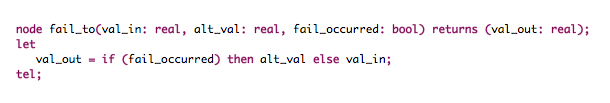
\includegraphics[width=1\textwidth]{images/fail_to.png}
  \vspace{-0.1in}
  \caption{AGREE Definition of a \textit{fail\_to} Fault}
  \label{fig:fail_to_node}
\end{figure}

%%%%%%% DANIELLE
%                     CHECK INTO MECHANICAL FAILURES

\item \textit{inverted\_fail} fault: This type of fault will be used on components which contain boolean output. It will simply take boolean input, negate it, and output the negated value. An examples of this is the Selector. See Figure~\ref{fig:inverted_fail_node}

\end{itemize}

\begin{figure}[h!]
  \centering
 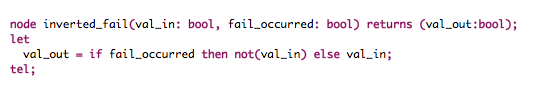
\includegraphics[width=1\textwidth]{images/inverted_fail.png}
  \vspace{-0.1in}
  \caption{AGREE Definition of a \textit{inverted\_fail} Fault}
  \label{fig:inverted_fail_node}
\end{figure}

While modeling these errors, the duration of the fault must also be taken into account. There are both permanent faults and transient faults. We defined an AGREE node called 
\begin{tt}
historically
\end{tt}
which will model the permanent faults based on whether transient faults are historically true. 

The following is a short summary of the failures defined in the fault model. 

\subsection{AADL Faults}
\begin{itemize}

\item Valves and Pumps: All valves and pumps have the possibility of a \textit{fail\_to} fault. This includes Green pump, Blue pump, Accumulator, and the Shutoff valves. 

\item  The Selector can also have a digital \textit{fail\_to} fault regarding the inputs from BSCU commanding to use Normal or Alternate means of pressure along with an \textit{inverted\_fail} fault which would change the boolean value that commands antiskid to activate. 

\end{itemize}

Given our understanding of the AADL system, the assumption was that permanent faults could be introduced into the system and we would still be able to prove our top level property. Upon connecting the faults into the WBS, it was shown that this top level property could not be proven using these permanent faults. Upon further reflection, it was clear why that was the case. 

In the AADL model, the Selector is situated between the pumps and the Blue\_Skid and Green\_Skid components. It's function is as follows: inputs are pump pressures (for Blue, Green, and Accumulator) and information from the BSCU regarding Normal or Alternate pressure. It selects between the Blue and the Green pump in this way. The output of the Selector is pressure of the Blue and Green pumps to the Blue\_Skid and Green\_Skid components respectively. The Blue\_Skid and Green\_Skid components also get a flag from BSCU. Blue\_Skid receives a flag with cmd\_alt while Green\_Skid gets the command cmd\_nor. This will cause those components to either output pressure (if their respective BSCU command is true) or output zero pressure (if the BSCU command is false). The pressure output from here goes directly to the wheel. For a clear picture of this organization, see Figure~\ref{fig:wbs_ima}.

Here is a case when the fault is \textit{fail\_to} and it is a failure of the Green\_Skid component. Previously in the system, the Selector received a command from BSCU to output Normal pressure (Green pump). This command was passed on to the Green\_Skid component along with positive green pressure. If the Green\_Skid component gets stuck at a value of zero for pressure, the output to the wheel is zero. The Blue\_Skid component gets no pressure from the Selector (it has already selected green pressure) and thus outputs no pressure to the wheel. 

Despite one transient failure, the tail end of the system is not designed to recover from this failure. A similar single point of failure is the Blue\_Skid component and the Selector. These faults cause system failure for the same reason. 

\subsection{Strengthening the Nominal Model}

To solve this issue, we added a component based on the Simulink model in \cite{Joshi05:Dasc}. This component, the Accumulator\_Valve, takes in the Blue pressure from the Selector and the Accumulator pressure. It also takes in a \textit{select\_Alternate} flag from the BSCU. The output of the Accumulator\_Valve goes directly to the Blue\_Skid component and is either the blue or the accumulator pressure. 

An additional piece we added was output to the BSCU from the wheel. The pressure at the wheel is sent to the BSCU to readjust system mode if needed. For instance, if the pressure at the wheel is zero from both blue and green skid components, then the BSCU has a chance to send a \textit{select\_Alternate} command over to the Accumulator\_Valve and turn on the accumulator pressure. We assume at this point that we will only use accumulator pressure and not switch back over to Normal mode. 

In order for this to solve the problem, the original top level contract needed to be revisited: 

\begin{tt}
If pedals are pressed and no skid occurs, then the brakes will receive pressure. 
\end{tt}

As it is stated, the added components will not solve the problem. There must be stateful information encoded into this contract. Thus it is changed to: 

\begin{tt}
If pedals are pressed in the previous state and in the current state and no skid occurs, then the brakes will receive pressure. 
\end{tt}

















%
%\input{experiments}
%
%\input{results}

%\input{related}

%\section{Conclusion}

We have developed an extension to the AADL language with tool support for formal analysis of system safety properties in the presence of faults. Faulty behavior is specified as an extension of the nominal model, allowing safety analysis and system implementation to be driven from a single common model. This new Safety Annex leverages the AADL structural model and nominal behavioral specification (using the AGREE annex) to propagate faulty component behaviors without the need to add separate propagation specifications to the model.   Next steps will include extensions to automate injection of Byzantine faults as well as automatic generation of fault trees.  For more details on the tool, models, and approach, see the technical report~\cite{SATechReport}.

\vspace{2 mm}
\noindent {\bf Acknowledgments.} This research was funded by NASA contract NNL16AB07T and the University of Minnesota College of Science and Engineering Graduate Fellowship.



%ACKNOWLEDGMENTS are optional
%TODO: Fill in for final version
\vspace{0.08in}


%\textbf{Acknowledgments:}
%This work was supported by

%We thank XXXX

\bibliographystyle{abbrv}
\bibliography{biblio}

% This ~ seems to fix an odd bibliography alignment issue
~

%\ifdefined\TECHREPORT
%\appendix
%
%\section{Appendix: Proof of Equivalence}
%\input{appendix}
%\fi

%\section{Appendix: GPCA CENTA Model}
%\label{appendix:gpcacenta}
%\begin{figure}[!ht]
%\begin{center}
%\includegraphics[scale=0.6]{images/sampled_pca.PNG} %[trim = 0 2 0 0, clip=true]{Comp}
%\caption{GPCA AGREE Properties modeled as a Timed Automata} \label{fig:samplepca}
%\end{center}
%\end{figure}

%\balancecolumns

\end{document}
